%%%%%%%%%%%%%%%%%%%%%%%%%%%%%%%%%%%%%%%%%%%%%%%%%%%%%%%%%%%%%%%%%%%%%%%%%%%%%%%%%%%%%%%%%%%%%%%%
%
% CS576 Written Question Template
%
% Acknowledgements:
% The original code is written by Prof. James Tompkin (james_tompkin@brown.edu).
% The second version is revised by Prof. Min H. Kim (minhkim@kaist.ac.kr).
%
% This is a LaTeX document. LaTeX is a markup language for producing 
% documents. Your task is to fill out this document, then to compile 
% it into a PDF document. 
%
% 
% TO COMPILE:
% > pdflatex thisfile.tex
%
% If you do not have LaTeX and need a LaTeX distribution:
% - Personal laptops (all common OS): www.latex-project.org/get/
% - We recommend latex compiler miktex (https://miktex.org/) for windows,
%   macTex (http://www.tug.org/mactex/) for macOS users.
%   And TeXstudio(http://www.texstudio.org/) for latex editor.
%   You should install both compiler and editor for editing latex.
%   The another option is Overleaf (https://www.overleaf.com/) which is 
%   an online latex editor.
%
% If you need help with LaTeX, please come to office hours. 
% Or, there is plenty of help online:
% https://en.wikibooks.org/wiki/LaTeX
%
% Good luck!
% Min and the CS576 staff
%
%%%%%%%%%%%%%%%%%%%%%%%%%%%%%%%%%%%%%%%%%%%%%%%%%%%%%%%%%%%%%%%%%%%%%%%%%%%%%%%%%%%%%%%%%%%%%%%%
%
% How to include two graphics on the same line:
% 
% \includegraphics[\width=0.49\linewidth]{yourgraphic1.png}
% \includegraphics[\width=0.49\linewidth]{yourgraphic2.png}
%
% How to include equations:
%
% \begin{equation}
% y = mx+c
% \end{equation}
% 
%%%%%%%%%%%%%%%%%%%%%%%%%%%%%%%%%%%%%%%%%%%%%%%%%%%%%%%%%%%%%%%%%%%%%%%%%%%%%%%%%%%%%%%%%%%%%%%%

\documentclass[11pt]{article}

\usepackage[english]{babel}
\usepackage[utf8]{inputenc}
\usepackage[colorlinks = true,
            linkcolor = blue,
            urlcolor  = blue]{hyperref}
\usepackage[a4paper,margin=1.5in]{geometry}
\usepackage{stackengine,graphicx}
\usepackage{fancyhdr}
\setlength{\headheight}{15pt}
\usepackage{microtype}
\usepackage{times}
\usepackage{booktabs}

% From https://ctan.org/pkg/matlab-prettifier
\usepackage[numbered,framed]{matlab-prettifier}

\frenchspacing
\setlength{\parindent}{0cm} % Default is 15pt.
\setlength{\parskip}{0.3cm plus1mm minus1mm}

\pagestyle{fancy}
\fancyhf{}
\lhead{Homework Writeup}
\rhead{CS576}
\rfoot{\thepage}

\date{}

\title{\vspace{-1cm}Homework 1: Zhang's Method and Plane Sweep}


\begin{document}
\maketitle
\vspace{-3cm}
\thispagestyle{fancy}

\section*{Instructions}
\begin{itemize}
  \item Describe any interesting decisions you made to write your algorithm.
  \item Show and discuss the results of your algorithm.
  \item Feel free to include code snippets, images, and equations.
  \item There is no page limit.
  
\end{itemize}

\section{In the beginning...}

The aim of this assignment was to implement Zhang's method for 'camera calibration' and then use 'Plane sweep stereo' technique for stereo matching. 

\section{For camera calibration}

The homography is the result of a nonlinear optimization. To solve it, we first optimise a function which is not physically meaningful, but can give us a closed-form solution which serves as a starting point for the nonlinear optimization with the physically meaningful cost function.

 The workflow for the first part consists of calculating homography using SVD, finding intrinsic parameters using matrices B and V, and then updating scale for every view to calculate extrinsic parameters. The rotation matrix estimated does not satisfy the properties of a rotation matrix in general. Hence, R is estimated using SVD. Finally, performing the nonlinear optimisation(MLE) concludes the portion of camera calibration.


\section{For Plane Sweep Stereo}

This part basically consists of 5 steps. First, obtain grayscale images. Second, form cost volume length * height *$ (max_d - min_d)$. Third, aggregation using imfilter function. Fourth, obtaining disparity map and finally, obtaining depth map from disparity.

See Equation~\ref{eq:one}.

\begin{equation}
depth = f*T/disparity
\label{eq:one}
\end{equation}


\section*{Interesting Implementation Detail}

I have attached the code snippet I wrote for Plane sweep stereo. I varied window size to find the one with best performance. Setting it to 13 gave the best performance.

\begin{lstlisting}[style=Matlab-editor]
  for d = 1 : length(d_vals);
    I2t = imtranslate(I2, [d 0]);
    C(:,:,d) = abs(I1 - I2t); 
    C(:,:,d) = imfilter(C(:,:,d), window);

  end

  [C_min, D] = min(C, [], 3);
  disparityMap = D + min_d;
  for i=1:size(disparityMap,1)
      for j=1:size(disparityMap,2)
          depthMap(i,j) = focalLength*baseline/disparityMap(i,j);
      end
  end
\end{lstlisting}

\section{Disparity and Depth maps for the two cases}

\begin{figure}[h]
    \centering
    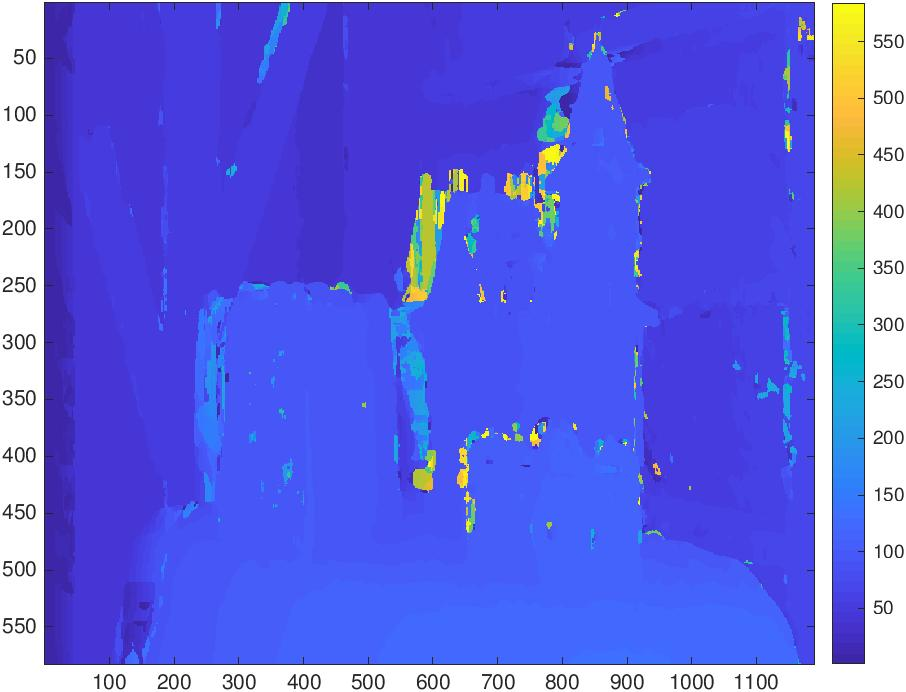
\includegraphics[width=7cm]{DisparityMap1.jpg}
    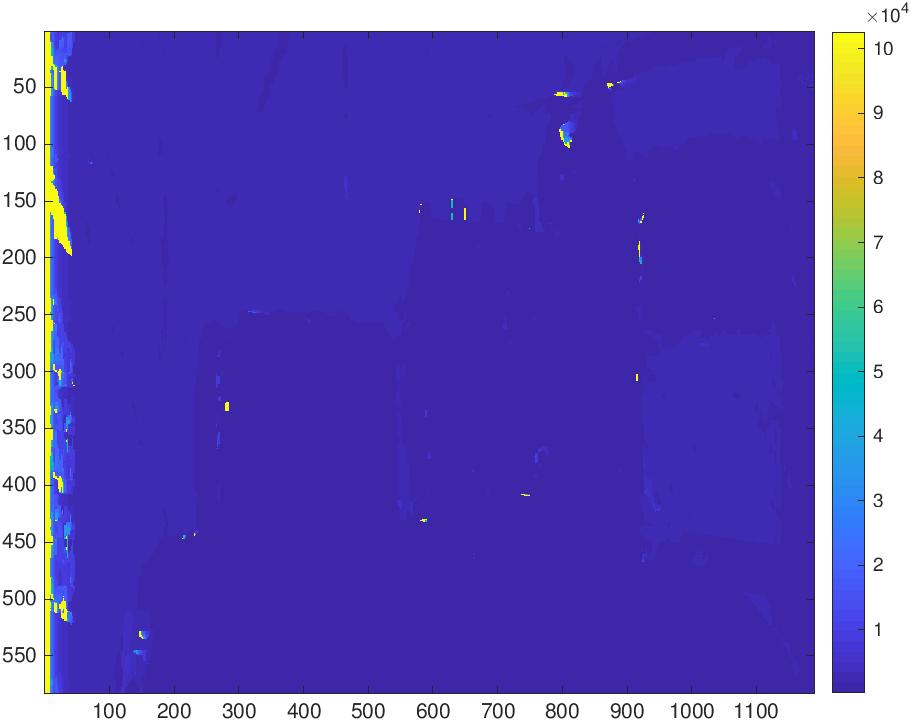
\includegraphics[width=7cm]{DepthMap1.jpg}
    \caption{\emph{Top:} DisparityMap1 \emph{Bottom:} DepthMap1}
    \label{fig:result1}
\end{figure}

\begin{figure}[h]
    \centering
    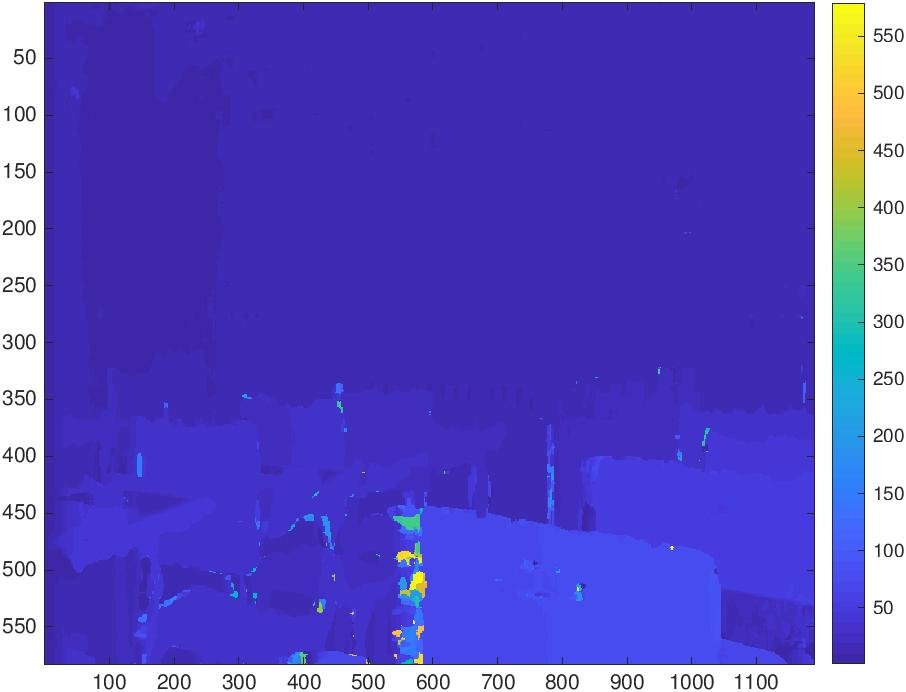
\includegraphics[width=7cm]{DisparityMap2.jpg}
    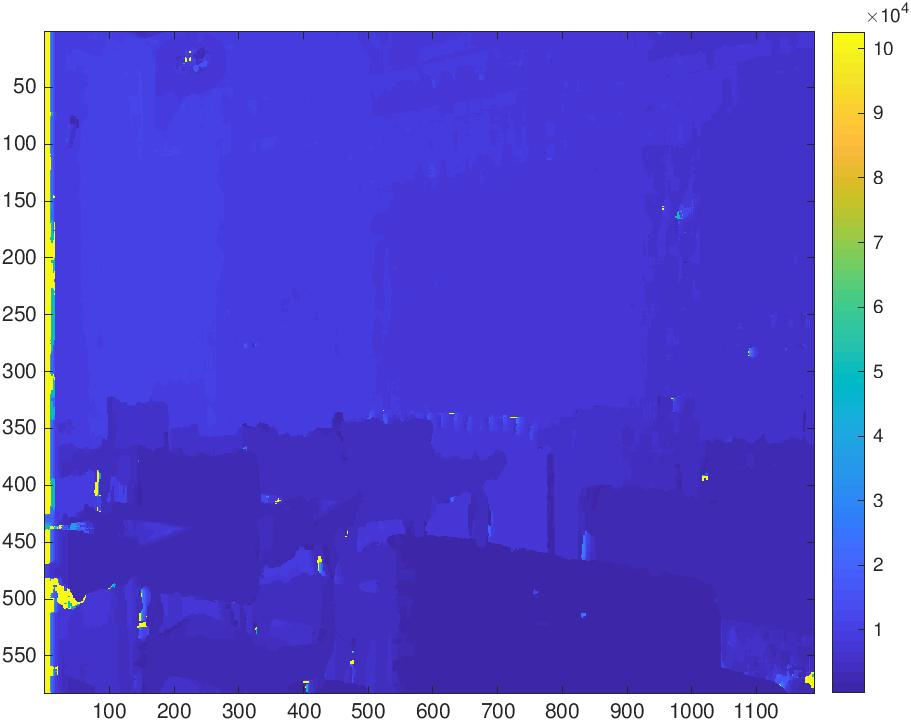
\includegraphics[width=7cm]{DepthMap2.jpg}
    \caption{\emph{Top:} DisparityMap2 \emph{Bottom:} DepthMap2}
    \label{fig:result2}
\end{figure}

\begin{figure}[h]
    \centering
    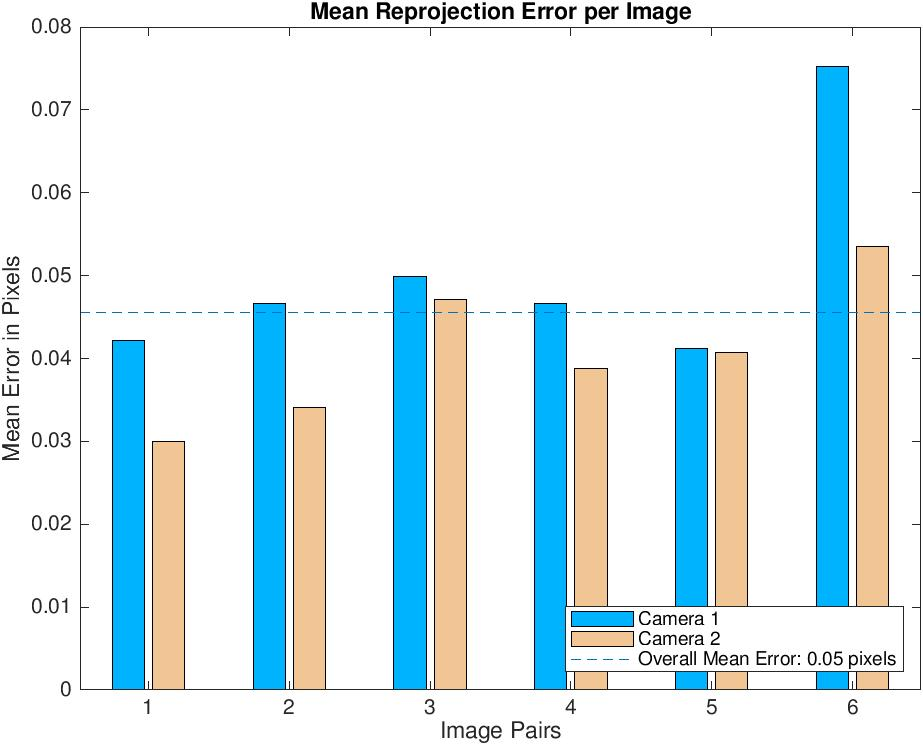
\includegraphics[width=9cm]{Mean_reprojection_error.jpg}
    %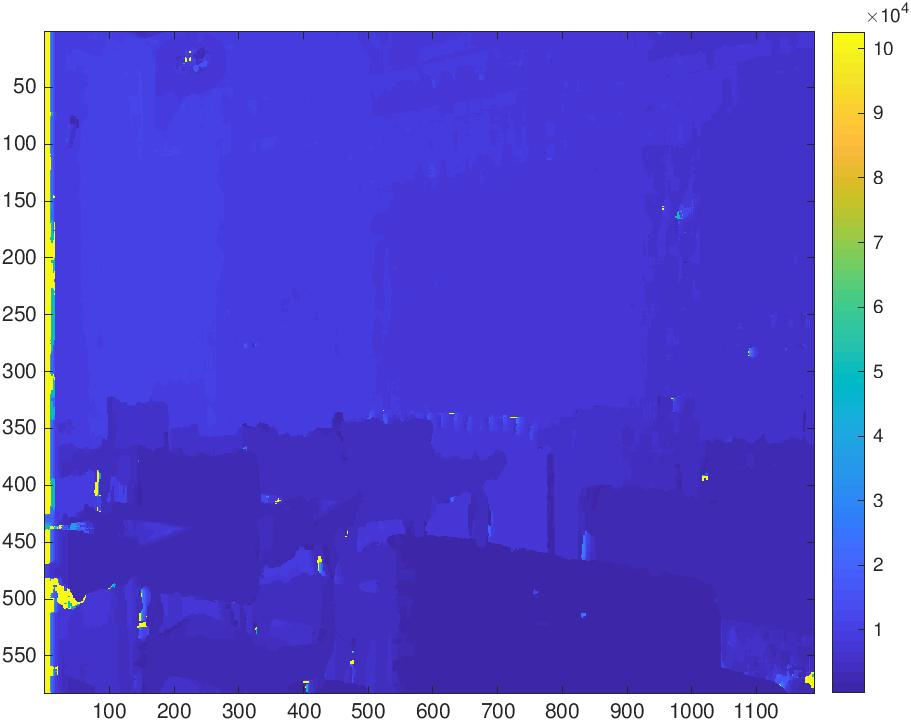
\includegraphics[width=5cm]{DepthMap2.jpg}
    \caption{Mean reprojection errors}
    \label{fig:result3}
\end{figure}

\begin{table}[h]
    \centering
    \begin{tabular}{lr}
        \toprule
        Original y-coordinate mean diff & Rectified y-coordinate mean diff \\
        \midrule
        11.9712 & 0.0563 \\
        14.7440 & 0.0274 \\
        \bottomrule
    \end{tabular}
    \caption{Y coordinate mean difference}
    \label{tab:table1}
\end{table}

\begin{table}[h]
    \centering
    \begin{tabular}{lr}
        \toprule
        Test no. & Depth Mean Difference(in mm)\\
        \midrule
        Test 1 & 485.87 \\
        Test 2 & 1471.74 \\
        \bottomrule
    \end{tabular}
    \caption{Depth mean difference}
    \label{tab:table2}
\end{table}

\end{document}